\chapter{Encryption over Cloud Model and its Process using Container}

\section{Swarm Manager}

\paragraph{\hspace{24pt}}
The job of a Swarm Manager is to send the plain text(unencrypted) code from the user a node which is running Docker Cryptography Container. Algorithms such as RSA and AES can be used for encryption of the file being uploaded.

\paragraph{\hspace{24pt}}
After encryption, the encrypted data is sent here. SSH protocol is used to handle the transaction of the files.

\paragraph{\hspace{24pt}}
After the transaction, the data is encrypted. However, it needs to be stored such that it is highly available. After the data is encrypted, it is sent back to a Gateway Manager.

\paragraph{\hspace{24pt}}
The data from the Gateway Manager is then sent to another node containing Storage manager(GlusterFS) This storage manager is connected to a new node containing multiple Docker containers. Then the encrypted data is distributed. GlusterFS is used to store the container cluster. By doing this, the encrypted files will be stored on multiple docker containers, thus forming a cluster of storage. This enables us to store data in chunks. This prevents the attacker from gaining the data since even if the node is compromised, the attacker will still have to target the containers. However, each container does not contain all the data as the data was distributed in previous steps. Here, having multiple containers helps.

\paragraph{\hspace{24pt}}
Similarly, we use the same process for decryption. First, the user downloads the required file, then the file is decrypted by the docker image and sent to the swarm manager, and from there the decrypted file is received.

\paragraph{\hspace{24pt}}
The following diagram shows the exact working model of Container Clustering using Dockers for Securing data on Cloud Servers or Storage.

\begin{figure}[htb]
\centering
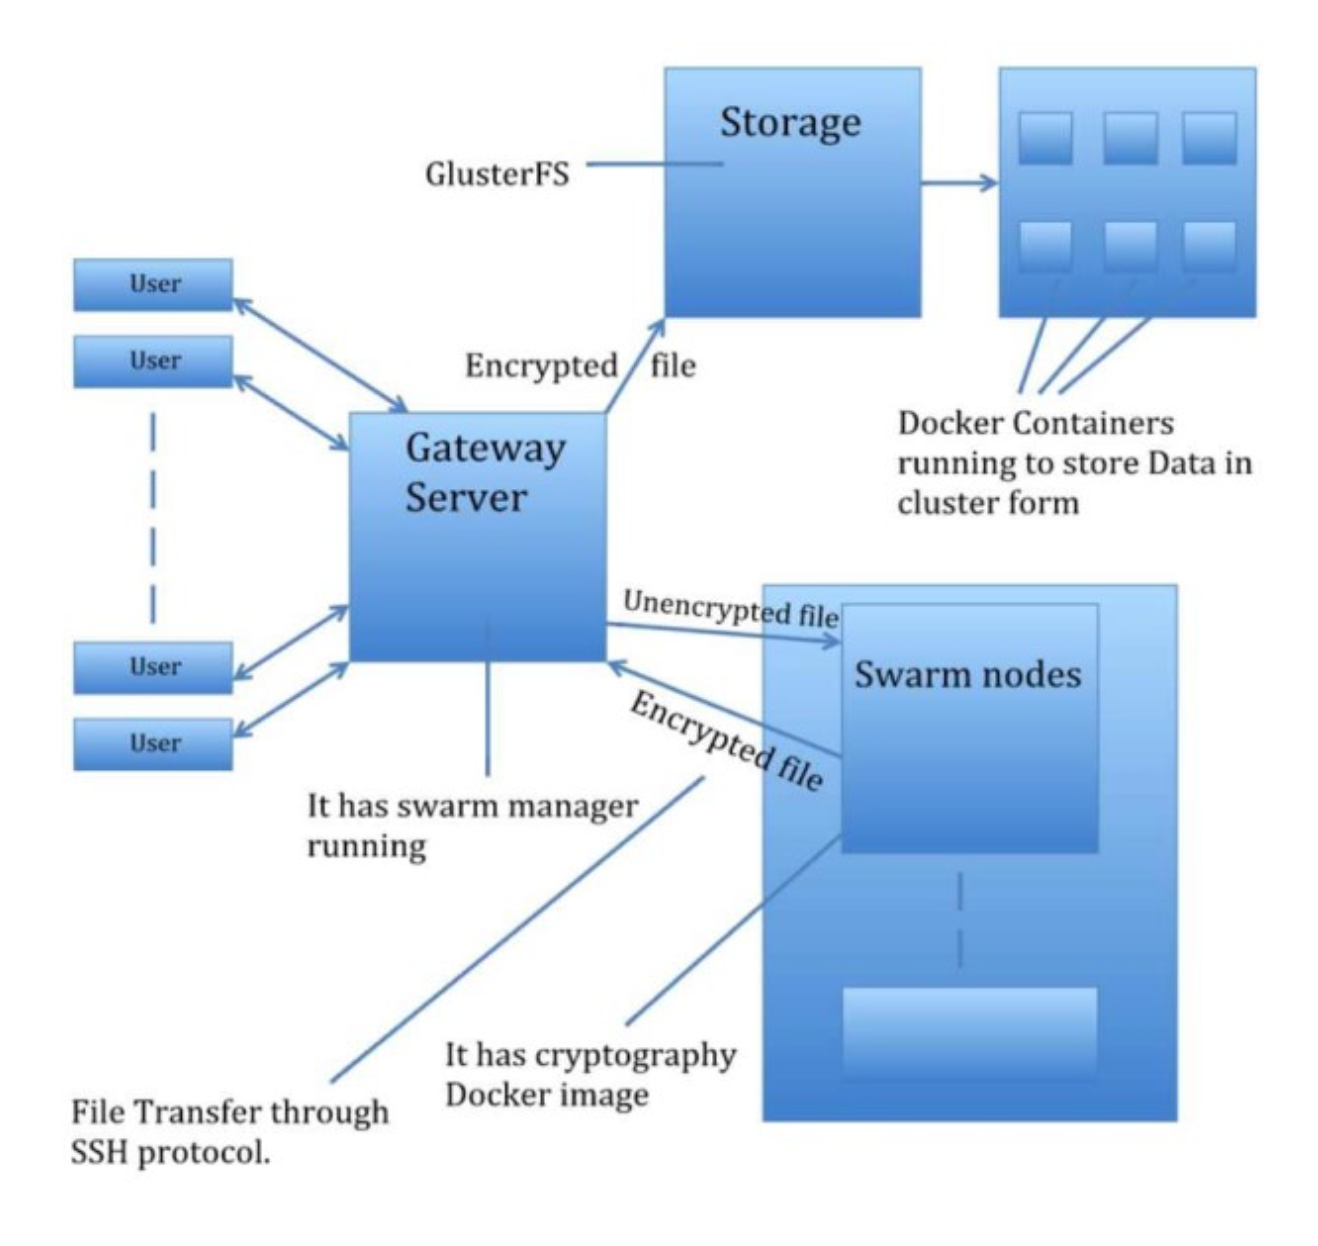
\includegraphics[width=10cm,height=6cm]{5-contents/8-encryption-over-cloud-model-and-its-process-using-container/images/container-clustering-docker.png} % e.g. insert ./image for image.png in the working directory, adjust scale as necessary
\caption{Container Clustering using Dockers Model}
\label{fig:label} % insert suitable label, this is used to refer to a fig from within the text as shown above
\end{figure}

\begin{figure}[htb]
\centering
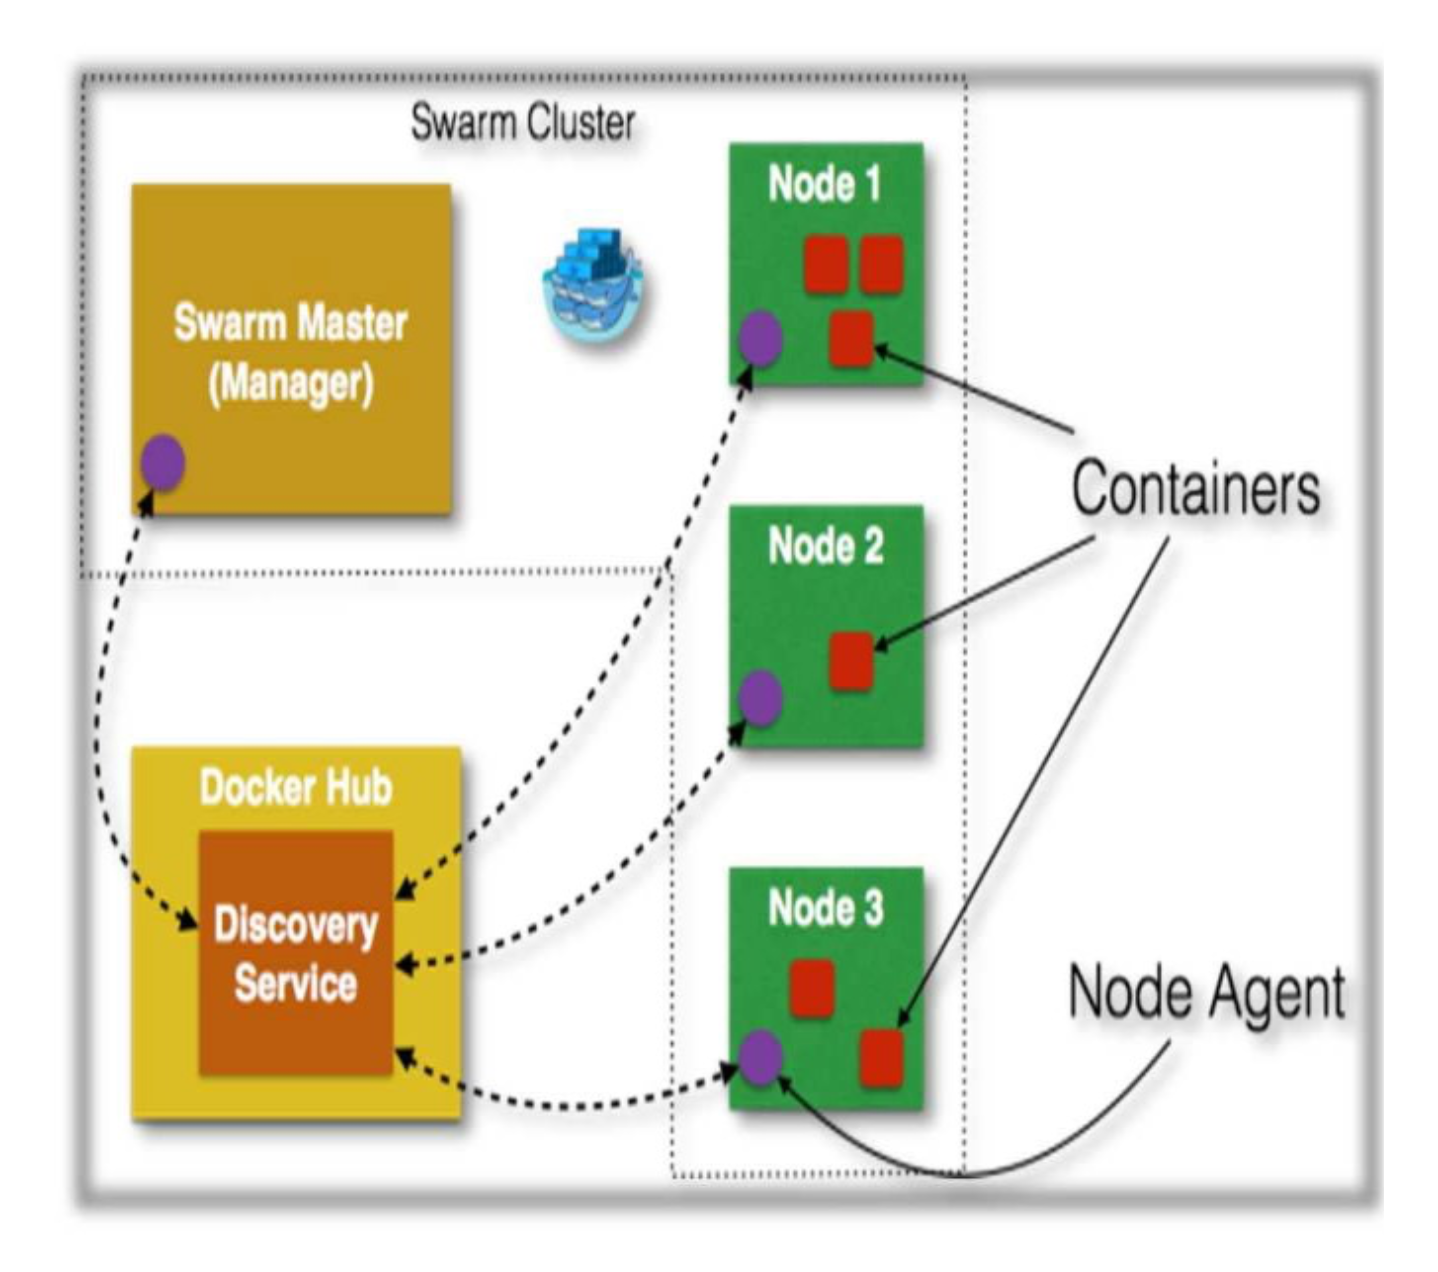
\includegraphics[width=10cm,height=6cm]{5-contents/8-encryption-over-cloud-model-and-its-process-using-container/images/docker-swarm-layout.png} % e.g. insert ./image for image.png in the working directory, adjust scale as necessary
\caption{Swarm Cluster Layout}
\label{fig:label} % insert suitable label, this is used to refer to a fig from within the text as shown above
\end{figure}

